\section{三类应用：语言、质量与毒性}

\subsection{语言识别}

语言识别的目标非常实用：先把非目标语言筛掉，再把算力留给真正关心的语言。对很多网页语料工程来说，这一步比“更聪明的模型”更重要，因为语料分散在多种语言、方言和代码混排里。

\begin{figure}[H]
\centering
\begin{tikzpicture}[every node/.style={font=\small, align=center}]
\node[draw, rounded corners, fill=green!12, minimum width=2.6cm, minimum height=0.9cm] (eng) at (0,0) {English};
\node[draw, rounded corners, fill=yellow!16, minimum width=2.8cm, minimum height=0.9cm] (mix) at (4,0) {code-switching};
\node[draw, rounded corners, fill=red!10, minimum width=2.6cm, minimum height=0.9cm] (other) at (8,0) {other language};
\draw[-{Latex[length=3mm]}, thick] (eng) -- (mix);
\draw[-{Latex[length=3mm]}, thick] (mix) -- (other);
\node[below=0.9cm of mix] {语言识别在边界处最难};
\end{tikzpicture}
\caption{语言识别的难点不是单语句子的“标准英语”，而是边界处的混合文本和低资源变体}
\end{figure}

\begin{knowledgebox}{语言识别的现实难题}
\begin{itemize}
    \item 短文本缺少上下文。
    \item 低资源语言样本少。
    \item code-switching 的语言边界并不稳定。
    \item 相近语言和方言容易互相混淆。
\end{itemize}
\end{knowledgebox}

课程里提到 fastText 语言识别支持 176 种语言，Dolma 则用 \texttt{p(English)} 作为一个简单门槛。这个门槛不一定很“科学”，但它够快，能把大批明显不是英语的页面先去掉。

\subsection{质量过滤}

质量过滤并不等于“语法正确”，它更像是在判断一页文本是否值得进入训练集。常见被剔除的对象包括模板页、广告页、低信息密度页、重复页、乱码页和明显的拼接页。

\begin{figure}[H]
\centering
\begin{tikzpicture}[every node/.style={font=\small, align=center}]
\node[draw, rounded corners, fill=green!10, minimum width=3.1cm, minimum height=0.95cm] (good) at (0,0) {high-quality\\Wikipedia / books};
\node[draw, rounded corners, fill=yellow!16, minimum width=3.1cm, minimum height=0.95cm] (mid) at (4.4,0) {mixed quality\\forums / blogs};
\node[draw, rounded corners, fill=red!10, minimum width=3.1cm, minimum height=0.95cm] (bad) at (8.8,0) {low quality\\spam / boilerplate};
\draw[-{Latex[length=3mm]}, thick] (good) -- (mid);
\draw[-{Latex[length=3mm]}, thick] (mid) -- (bad);
\end{tikzpicture}
\caption{质量过滤是沿着“信息密度”而不是“语法正确性”做粗粒度排序}
\end{figure}

\begin{importantbox}{质量过滤的本质}
它不是定义“完美文档”，而是决定“哪些数据更值得被训练”。只要能持续过滤掉最差的那一截，收益通常就会很明显。
\end{importantbox}

\begin{figure}[H]
\centering
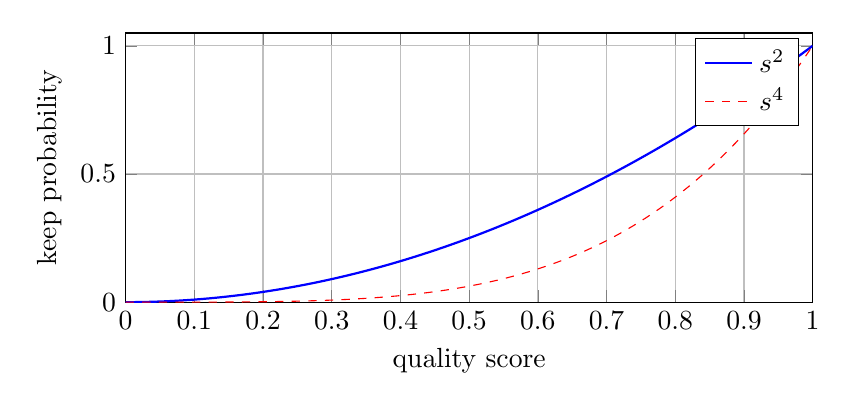
\begin{tikzpicture}
\begin{axis}[
    width=0.85\textwidth,
    height=5cm,
    xlabel={quality score},
    ylabel={keep probability},
    ymin=0, ymax=1.05,
    xmin=0, xmax=1,
    grid=both,
]
\addplot[blue, thick, domain=0:1, samples=100] {x^2};
\addplot[red, dashed, domain=0:1, samples=100] {x^4};
\legend{$s^2$, $s^4$}
\end{axis}
\end{tikzpicture}
\caption{像 GPT-3 这样的随机保留策略，可以用更陡的曲线把高分样本保留下来、低分样本快速压下去}
\end{figure}

GPT-3、LLaMA/RedPajama、phi-1 的差异在于正负样本选择不同，但骨架是一样的：先训练一个轻量分类器或打分器，再按分数筛选。phi-1 的有趣之处在于，它把“教育价值”作为过滤准则，用教材和高质量合成样本去筛大规模代码数据。

\subsection{毒性过滤}

毒性过滤是更直接的治理场景。Dolma 使用 Jigsaw Toxic Comments 数据训练轻量分类器，把评论分成 toxic、severe\_toxic、obscene、threat、insult、identity\_hate 等类，再按需求过滤或标记。

\begin{figure}[H]
\centering
\begin{tikzpicture}[node distance=1.2cm, every node/.style={font=\small, align=center}]
\node[draw, rounded corners, fill=green!10, minimum width=3.1cm, minimum height=0.85cm] (train) {labeled toxic comments};
\node[draw, rounded corners, fill=yellow!16, below=of train, minimum width=3.1cm, minimum height=0.85cm] (clf) {train fastText classifier};
\node[draw, rounded corners, fill=blue!14, below=of clf, minimum width=3.1cm, minimum height=0.85cm] (pred) {predict on web crawl};
\node[draw, rounded corners, fill=red!10, below=of pred, minimum width=3.1cm, minimum height=0.85cm] (act) {filter / flag / downweight};
\draw[-{Latex[length=3mm]}, thick] (train) -- (clf);
\draw[-{Latex[length=3mm]}, thick] (clf) -- (pred);
\draw[-{Latex[length=3mm]}, thick] (pred) -- (act);
\end{tikzpicture}
\caption{毒性过滤的典型管线：用带标签数据训练轻量分类器，再把它应用到网页级数据上}
\end{figure}

\begin{warningbox}{毒性过滤的坑}
误杀经常出现在短文本、引号引用、讽刺、代码混排和方言里。一个看似“更严格”的分类器，可能只是把更多正常内容误删掉。
\end{warningbox}

